% !Tex program = pdflatex
% 第 10 章: 正规算子的结构理论 Chap 10: Structure Theory for Normal Operator
\ifx\allfiles\undefined
\documentclass{note}
\setcounter{chapter}{+9}
\begin{document}
\fi
\chapter{正规算子的结构理论}
\section{线性算子的伴随}
先来回顾一下算子伴随: $\mathcal{B}$ 和 $\mathcal{C}$ 分别为线性空间 $V$ 和 $W$ 的定序基, $V^*$ 和 $W^*$ 分别为 $V$ 和 $W$ 的对偶空间, $\mathcal{B}^*$ 和 $\mathcal{C}^*$ 分别为 $\mathcal{B}$ 和 $\mathcal{C}$ 的对偶基, 对给定的线性变换 $\tau\in\mathcal{L}(V,W)$, 有算子伴随 $\tau^{\times}:W^*\rightarrow V^*$, $g\mapsto \tau^{\times}=g\circ\tau$, 线性变换在定序基上与其算子伴随在对偶基上的表示存在关系: $[\tau]_{\mathcal{B}\mathcal{C}}=[\tau^{\times}]_{\mathcal{C}^*\mathcal{B}^*}$.
\begin{center}
    \begin{tikzpicture}
        \node(1)at(-2,2){$V$};
        \node(2)at(2,2){$W$};
        \node(3)at(0,-2){$F$};
        \draw[->](1)--(2)node[midway]{$\tau$};
        \draw[->](2)--(3)node[midway]{$g$};
        \draw[->](1)--(3)node[midway]{$\tau^{\times}=g\circ\tau$};
    \end{tikzpicture}
\end{center}

下面来定义另一种伴随: 对于有限维内积向量空间 $V$ 和 $W$, $\dim V=n$, $\dim W=m$, Riesz 映射 $\mathcal{R}_V:V^*\rightarrow V$, $\mathcal{R}_W:W^*\rightarrow W$, $\because\mathcal{R}_W$ 为共轭同构, $\therefore$ 有其逆同构 $\mathcal{R}_W^{-1}$, 从而有映射 $\tau^*=\mathcal{R}_V\circ\tau^{\times}\circ\mathcal{R}_W$.
\begin{center}
    \begin{tikzpicture}
        \node(1)at(-2,2){$V$};
        \node(2)at(2,2){$W$};
        \node(3)at(-2,-2){$V^*$};
        \node(4)at(2,-2){$W^*$};
        \node(6)at(3,3){$u$};
        \node(8)at(3,-3){$\mathcal{R}_W^{-1}(u)$};
        \node(7)at(-3,-3){$\tau^{\times}(\mathcal{R}_W^{-1}(u))$};
        \node(5)at(-3,3){$\mathcal{R}_V(\tau^{\times}(\mathcal{R}_W^{-1}(u)))$};
        \draw[->](1.north east)--(2.north west)node[midway]{$\tau$};
        \draw[->](3)--(1)node[midway]{$\mathcal{R}_V$};
        \draw[->](4)--(2)node[midway]{$\mathcal{R}_W$};
        \draw[->](4)--(3)node[midway]{$\tau^{\times}$};
        \draw[dashed,->](2.south west)--(1.south east)node[midway]{$\tau^*$?};
        \draw[|->](7)--(5);
        \draw[|->](8)--(6);
        \draw[|->](8)--(7);
    \end{tikzpicture}
\end{center}

\begin{thm}[(课本定理 10.1)]\label{thm-10.1}
    \begin{itemize}
        \item[(1)] $\tau^*$ 为线性变换, 即 $\tau^*\in\mathcal{L}(W,V)$.
        \item[(2)] $\langle v,\tau^*(w)\rangle=\langle\tau(v),w\rangle$, 称 $\tau^*$ 为 $\tau$ 的伴随.
        \item[(3)] $[\tau]_{\mathcal{BC}}=[\tau^*]_{\mathcal{CB}}^{\dagger}$.
    \end{itemize}
\end{thm}
\begin{pf}
    \begin{itemize}
        \item[(1)] $\tau^*=\mathcal{R}_V\circ\tau^{\times}\circ\mathcal{R}_W^{-1}:W\rightarrow V$.\\
        $\forall u_1,u_2\in W$, $\tau^*(ru_1+tu_2)=\mathcal{R}_V\circ\tau^{\times}\circ\mathcal{R}_W^{-1}(ru_1+tu_2)=\mathcal{R}_V\circ\tau^{\times}(\mathcal{R}_W^{-1}(ru_1+tu_2))=\mathcal{R}_V\circ\tau^{\times}(\bar{r}\mathcal{R}_W^{-1}(u_1)+\bar{t}\mathcal{R}_W^{-1}(u_2))=\mathcal{R}_V(\tau^{\times}(\bar{r}\mathcal{R}_W^{-1}(u_1)+\bar{t}\mathcal{R}_W^{-1}(u_2)))=\mathcal{R}_V(\bar{r}\tau^{\times}(\mathcal{R}_W^{-1}(u_1))+\bar{t}\tau^{\times}(\mathcal{R}_W^{-1}(u_2)))=r\mathcal{R}_V(\tau^{\times}(\mathcal{R}_W^{-1}(u_1)))+t\mathcal{R}_V(\tau^{\times}(\mathcal{R}_W^{-1}(u_2)))=r\tau^*(u_1)+t\tau^*(u_2)$, 其中利用了引理 \ref{inverse Riesz conjugate linear}, 得证.
        \item[(2)] $\forall v\in V$, $\forall w\in W$, $\langle v,\tau^*(w)\rangle=\langle v,\mathcal{R}_V(\tau^{\times}\circ\mathcal{R}_W^{-1}(w))\rangle=\tau^{\times}\circ\mathcal{R}_W^{-1}(w)(v)=\mathcal{R}_W^{-1}(w)\circ\tau(v)=\mathcal{R}_W^{-1}(w)(\tau(v))=\langle\tau(v),w\rangle$.
        \item[(3)] 设 $V$ 的正交归一基 $\mathcal{B}=\{b_1,\cdots,b_n\}$, $W$ 的正交归一基 $\mathcal{C}=\{c_1,\cdots,c_n\}$.\\
        $[\tau]_{\mathcal{BC}}=\begin{pmatrix}
            [\tau(b_1)]_{\mathcal{C}}&\cdots&[\tau(b_n)]_{\mathcal{C}}
        \end{pmatrix}$, $[\tau^*]_{\mathcal{CB}}=\begin{pmatrix}
            [\tau(c_1)]_{\mathcal{B}}&\cdots&[\tau(c_m)]_{\mathcal{B}}
        \end{pmatrix}$.\\
        设 $[\tau(b_i)]_{\mathcal{C}}=\begin{pmatrix}
            \alpha_{1i}\\
            \vdots\\
            \alpha_{mi}
        \end{pmatrix}$, $\tau(b_i)=\sum_{k=1}^m\alpha_{ki}c_k$, $\langle\tau(b_i),c_j\rangle=\langle\sum_{k=1}^m\alpha_{ki}c_k,c_j\rangle=\sum_{k=1}^m\alpha_{ki}\langle c_k,c_j\rangle=\sum_{k=1}^m\alpha_{ki}\delta_{kj}=\alpha_{ji}$.\\
        同理, 设 $[\tau^*(c_j)]_{\mathcal{B}}=\begin{pmatrix}
            \beta_{1j}\\
            \vdots\\
            \beta_{nj}
        \end{pmatrix}$, $\tau^*(c_j)=\sum_{k=1}^n\beta_{kj}b_k$, $\langle \tau^*(c_j),b_i\rangle=\langle\sum_{k=1}^n\beta_{kj}b_k,b_i\rangle=\sum_{k=1}^n\beta_{kj}\langle b_k,b_i\rangle=\sum_{k=1}^n\beta_{kj}\delta_{ki}=\beta_{ij}$.\\
        又 $\because\langle\tau(b_i),c_j\rangle=\langle b_i,\tau^*(c_j)\rangle=\overline{\langle\tau^*(c_j),b_i\rangle}$, $\therefore\alpha_{ji}^*=\beta_{ij}\Longrightarrow[\tau]_{\mathcal{BC}}=[\tau^*]_{\mathcal{CB}}^{\dagger}$.
    \end{itemize}
\end{pf}

\begin{cor}\label{inverse Riesz conjugate linear}
    Riesz 映射的逆 $\mathcal{R}^{-1}$ 共轭线性.
\end{cor}
\begin{pf}
    $\forall x_1,x_2\in V$, $\exists f_1=\mathcal{R}^{-1}(x_1),f_2=\mathcal{R}^{-1}(x_2)\in V^*$, s.t. $\forall v\in V$, $f_1(v)=\langle v,x_1\rangle$, $f_2(v)=\langle v,x_2\rangle$\\
    $\Longrightarrow\forall\bar{r},\bar{t}\in F$, $(\bar{r}\mathcal{R}^{-1}(x_1)+\bar{t}\mathcal{R}^{-1}(x_2))(v)=(\bar{r}f_1+\bar{t}f_2)(v)=\bar{r}f_1(v)+\bar{t}f_2(v)=\bar{r}\langle v,x_1\rangle+\bar{t}\langle v,x_2\rangle=\langle v,rx_1\rangle+\langle v,tx_2\rangle=\langle v,rx_1+tx_2\rangle=\mathcal{R}^{-1}(rx_1+rx_2)(v)$\\
    $\Longrightarrow\mathcal{R}^{-1}(rx_1+tx_2)=\bar{r}\mathcal{R}^{-1}(x_1)+\bar{t}\mathcal{R}^{-1}(x_2)$.
\end{pf}

$\because[\tau]_{\mathcal{BC}}=[\tau^{\times}]_{\mathcal{C}^*\mathcal{B}^*}^T$, $[\tau]_{\mathcal{BC}}=[\tau^*]_{\mathcal{CB}}^{\dagger}$, $\therefore[\tau^{\times}]_{\mathcal{C}^*\mathcal{B}^*}=\overline{[\tau^*]_{\mathcal{CB}}}$. 当然这也可用类似定理 \ref{thm-10.1} (3) 的证明方法证明:
\begin{pf}
    $[\tau^{\times}]_{\mathcal{C}^*\mathcal{B}^*}=\begin{pmatrix}
        [\tau^{\times}(c_1^*)]_{\mathcal{B}^*}&\cdots&[\tau^{\times}(c_n^*)]_{\mathcal{B}^*}
    \end{pmatrix}$, $[\tau^*]_{\mathcal{CB}}=\begin{pmatrix}
        [\tau^*(c_1)]_{\mathcal{B}^*}&\cdots&[\tau^*(c_n)]_{\mathcal{B}}
    \end{pmatrix}$,\\
    设 $[\tau^{\times}(c_i^*)]_{\mathcal{B}^*}=\begin{pmatrix}
        \alpha_{1i}\\
        \vdots\\
        \alpha_{ni}
    \end{pmatrix}$, 则 $\tau^{\times}(c_i^*)=\sum_{k=1}^n\alpha_{ki}b_k^*$.\\
    设 $[\tau^*(c_i)]_{\mathcal{B}}=\begin{pmatrix}
        \beta_{1i}\\
        \vdots\\
        \beta_{mi}
    \end{pmatrix}$, 则 $\tau^*(c_i)=\sum_{k=1}^m\beta_{ki}b_k$.\\
    一方面, $\because\mathcal{R}_W^{-1}(c_i)(c_j)=\langle c_j,c_i\rangle=\delta_{ij}$, $\therefore\mathcal{R}_V(c_i)=c_i^*$\\
    $\Longrightarrow\langle b_j,\tau^*(c_i)\rangle=\langle b_j,\mathcal{R}_V\circ\tau^{\times}\circ\mathcal{R}_W^{-1}(c_i)\rangle=\langle b_j,\mathcal{R}_V(\tau^{\times}(\mathcal{R}_W^{-1}(c_i)))\rangle=\langle b_j,\mathcal{R}_V(\tau^{\times}(c_i^*))\rangle=\tau^{\times}(c_i^*)(b_j)=\left(\sum_{k=1}^n\alpha_{ki}b_k^*\right)(b_j)=\sum_{k=1}^n\alpha_{ki}b_k^*(b_j)=\sum_{k=1}^n\alpha_{ki}\delta_{jk}=\alpha_{ji}$;\\
    另一方面, $\langle b_j,\tau^*(c_i)\rangle=\langle b_j,\sum_{k=1}^m\beta_{ki}b_k\rangle=\sum_{k=1}^m\overline{\beta_{ki}}\langle b_j,b_k\rangle=\sum_{k=1}^m\overline{\beta_{ki}}\delta_{jk}=\overline{\beta_{ji}}$.\\
    故 $\alpha_{ji}=\overline{\beta_{ji}}$, 得证.
\end{pf}

\begin{thm}[(课本定理 10.2)]
    $V,W$ 为有限维内积向量空间, $\forall\sigma,\tau\in\mathcal{L}(V,W)$, $\forall r\in F$,
    \begin{itemize}
        \item[(1)] $(\sigma+\tau)^*=\sigma^*+\tau^*$.
        \item[(2)] $(r\tau)^*=\bar{r}\tau^*$.
        \item[(3)] $\tau^{**}=\tau$.
        \item[(4)] 若 $V=W$, 则 $(\tau\circ\sigma)^*=\sigma^*\circ\tau^*$.
        \item[(5)] $V=W$, 若 $\tau$ 可逆, 则 $(\tau^{-1})^*=(\tau^*)^{-1}$.
        \item[(6)] $V=W$, $p(x)\in\mathbb{R}[x]$, 则 $p(\tau)^*=p(\tau^*)$.
        \item[(7)] $S$ 是 $V$ 的子空间, $\tau\in\mathcal{L}(V)$, 则 $S$ 是 $\tau$ 的不变子空间 $\Longleftrightarrow S^{\perp}$ 是 $\tau^*$ 的不变子空间.
    \end{itemize}
\end{thm}
\begin{pf}
    \begin{itemize}
        \item[(1)] $\forall u\in W$, $\forall v\in V$, $\langle v,(\sigma+\tau)^*(u)\rangle=\langle(\sigma+\tau)(v),u\rangle=\langle\sigma(v)+\tau(v),u\rangle=\langle\sigma(v),u\rangle+\langle\tau(v),u\rangle=\langle v,\sigma^*(u)\rangle+\langle v,\tau^*(u)\rangle=\langle v,\sigma^*(u)+\tau^*(u)\rangle=\langle v,(\sigma^*+\tau^*)(u)\rangle\Longrightarrow(\sigma+\tau)^*(u)=(\sigma^*+\tau^*)(u)\Longrightarrow(\sigma+\tau)^*=\sigma^*+\tau^*$.
        \item[(2)] $\forall u\in W$, $\forall v\in V$, $\langle v,(r\tau)^*(u)\rangle=\langle r\tau(v),u\rangle=r\langle\tau(v),u\rangle=r\langle v,\tau^*(u)\rangle=\langle v,\bar{r}\tau^*(u)\rangle\Longrightarrow(r\tau)^*(u)=\bar{r}\tau(u)\Longrightarrow(r\tau)^*=\bar{r}\tau^*$.
        \item[(3)] $\forall u\in W$, $\forall v\in V$, $\langle u,\tau^{**}(v)\rangle=\langle u,(\tau^*)^*(v)\rangle=\langle\tau^*(u),v\rangle=\overline{\langle v,\tau^*(u)\rangle}=\overline{\langle\tau(v),u\rangle}=\langle u,\tau(v)\rangle\Longrightarrow\tau^{**}(v)=\tau(v)\Longrightarrow\tau^{**}=\tau$.
        \item[(4)] $\forall v\in V$, $\forall u\in W$, $\langle u,(\tau\circ\sigma)^*(v)\rangle=\langle(\tau\circ\sigma)(u),v\rangle=\langle\tau(\sigma(u)),v\rangle=\langle\sigma(u),\tau^*(v)\rangle=\langle u,\sigma^*(\tau^*(v))\rangle=\langle u,(\sigma^*\circ\tau^*)(v)\rangle\Longrightarrow(\tau\circ\sigma)^*(v)=(\sigma^*\circ\tau^*)(v)\Longrightarrow(\tau\circ\sigma)^*=\sigma^*\circ\tau^*$.
        \begin{center}
            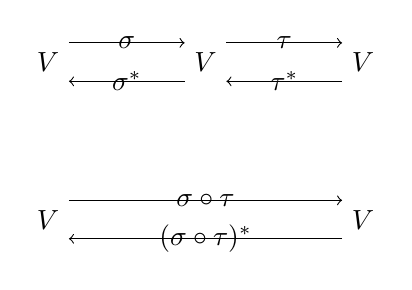
\begin{tikzpicture}
                \node(1)at(-2,1){$V$};
                \node(2)at(0,1){$V$};
                \node(3)at(2,1){$V$};
                \draw[->](1.north east)--(2.north west)node[midway]{$\sigma$};
                \draw[->](2.north east)--(3.north west)node[midway]{$\tau$};
                \draw[->](3.south west)--(2.south east)node[midway]{$\tau^*$};
                \draw[->](2.south west)--(1.south east)node[midway]{$\sigma^*$};

                \node(4)at(-2,-1){$V$};
                \node(5)at(2,-1){$V$};
                \draw[->](4.north east)--(5.north west)node[midway]{$\sigma\circ\tau$};
                \draw[->](5.south west)--(4.south east)node[midway]{$(\sigma\circ\tau)^*$};
            \end{tikzpicture}
        \end{center}
        \item[(5)] $(\tau^{-1})^*\circ\tau^*=(\tau\circ\tau^{-1})^*=1_V^*=1_V\Longrightarrow(\tau^{-1})^*=(\tau^*)^{-1}$.
        \begin{center}
            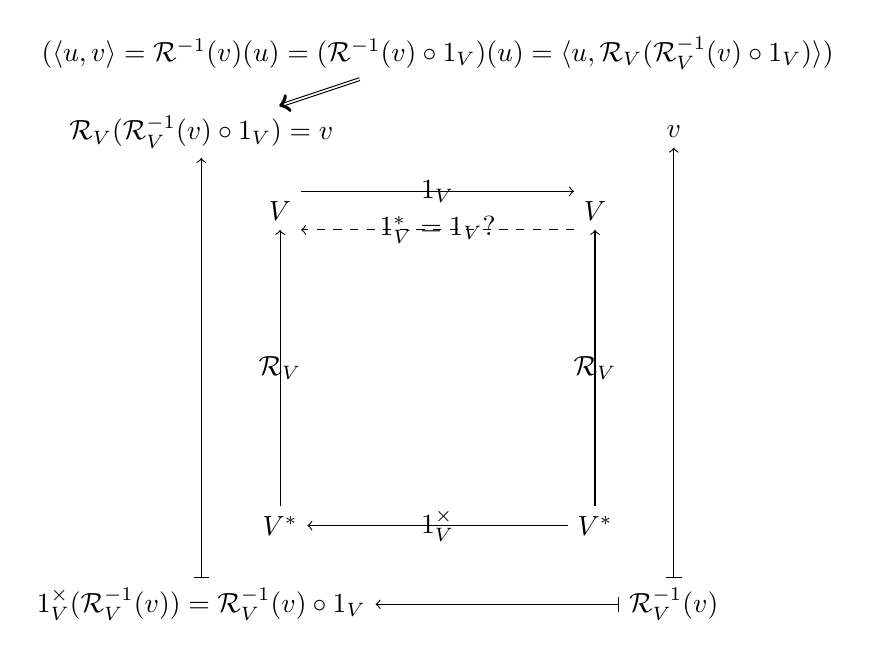
\begin{tikzpicture}
                \node(1)at(-2,2){$V$};
                \node(2)at(2,2){$V$};
                \node(3)at(-2,-2){$V^*$};
                \node(4)at(2,-2){$V^*$};
                \node(6)at(3,3){$v$};
                \node(8)at(3,-3){$\mathcal{R}_V^{-1}(v)$};
                \node(7)at(-3,-3){$1_V^{\times}(\mathcal{R}_V^{-1}(v))=\mathcal{R}_V^{-1}(v)\circ 1_V$};
                \node(5)at(-3,3){$\mathcal{R}_V(\mathcal{R}_V^{-1}(v)\circ 1_V)=v$};
                \draw[->](1.north east)--(2.north west)node[midway]{$1_V$};
                \draw[->](3)--(1)node[midway]{$\mathcal{R}_V$};
                \draw[->](4)--(2)node[midway]{$\mathcal{R}_V$};
                \draw[->](4)--(3)node[midway]{$1_V^{\times}$};
                \draw[dashed,->](2.south west)--(1.south east)node[midway]{$1_V^*=1_V$?};
                \draw[|->](7)--(5);
                \draw[|->](8)--(6);
                \draw[|->](8)--(7);
                \node(9)at(0,4){$(\because\langle u,v\rangle=\mathcal{R}^{-1}(v)(u)=(\mathcal{R}^{-1}(v)\circ 1_V)(u)=\langle u,\mathcal{R}_V(\mathcal{R}_V^{-1}(v)\circ 1_V)\rangle)$};
                \draw[->,double](9)--(5);
            \end{tikzpicture}
        \end{center}
        \item[(6)] $(\tau\circ\tau)^*=\tau^*\circ\tau^*$, $(\tau^k)^*=(\tau^*)^k$.\\
        若 $r\in\mathbb{R}$, 则 $(r\tau)^*=rt^*$, $(r\tau^k)^*=r(\tau^*)^k$\\
        $\Longrightarrow(p(\tau))^*=p(\tau^*)$.
        \item[(7)] ``$\Longrightarrow$'': $\because S$ 是 $\tau$ 的不变子空间, $\therefore\tau(S)\subseteq S$.\\
        $\forall v\in S^{\perp}$, $\forall u\in S$, $\tau(u)\in S\Longrightarrow\langle u,\tau^*(v)\rangle=\langle\tau(u),v\rangle=0\Longrightarrow\tau^*(v)\in S^{\perp}\Longrightarrow S^{\perp}$ 是 $\tau^*$ 的不变子空间.

        ``$\Longleftarrow$'': $\because S^{\perp\perp}=S$, 故同理得证.
    \end{itemize}
\end{pf}

\begin{thm}[(课本定理 10.3)]
    $V,W$ 为有限维内积向量空间, $\tau\in\mathcal{L}(V,W)$, 则
    \begin{itemize}
        \item[(1)] $\ker\tau^*=(\im\tau)^{\perp}$, 等价地, $\im\tau^*=(\ker\tau)^{\perp}$.
        \item[(2)] $\ker\tau^*\tau=\ker\tau$, $\ker\tau\tau^*=\ker\tau^*$.
        \item[(3)] $\im\tau^*\tau=\im\tau^*$, $\im\tau\tau^*=\im\tau$.
        \item[(4)] $\rho_{ST}^*=\rho_{T^{\perp}S^{\perp}}$.
    \end{itemize}
\end{thm}
\begin{pf}
    \begin{itemize}
        \item[(1)] $\forall w\in\im\tau$, $\exists u\in V$, s.t. $w=\tau(u)$.\\
        $v\in\ker\tau^*\Longleftrightarrow\tau^*(v)=0\Longleftrightarrow\langle w,v\rangle=\langle\tau(u),v\rangle=\langle u,\tau^*(v)\rangle=\langle u,0\rangle=0\Longleftrightarrow v\in(\im\tau)^{\perp}$, 故 $\ker\tau^*=(\im\tau)^{\perp}$.

        $\forall w\in\ker\tau$, $\Longleftrightarrow$$\tau(w)=0\in W$.\\
        $v\in\im\tau^*\Longleftrightarrow\exists u\in W$, s.t. $\tau^*(u)=v\Longleftrightarrow\langle w,v\rangle=\langle w,\tau^*(u)\rangle=\langle\tau(w),u\rangle=\langle 0,u\rangle=0\Longleftrightarrow v\in(\ker\tau)^{\perp}$, 故 $\im\tau^*=(\ker\tau)^{\perp}$.
        \item[(2)] $\forall v\in\ker\tau\tau^*$, $\tau^*\tau(v)=0\Longrightarrow\langle v,\tau^*\tau(v)\rangle=0\Longleftrightarrow\langle\tau(v),\tau(v)\rangle=0\Longrightarrow\tau(v)=0\Longleftrightarrow v\in\ker\tau$, 故 $\ker\tau^*\tau\subseteq\ker\tau$.

        $\forall v\in\ker\tau$, $\tau(v)=0\Longrightarrow\tau^*\tau(v)=0\Longleftrightarrow v\in\ker\tau^*\tau$, 故 $\ker\tau\subseteq\ker\tau^*\tau$.

        综上, $\ker\tau^*\tau=\ker\tau$.

        同理, $\ker\tau\tau^*=\ker\tau^*$.
        \item[(3)] $\forall v\in\im\tau^*\tau$, $\exists u\in V$, s.t. $u=\tau^*\tau(v)=\tau^*(\tau(v))$, 即 $\exists w=\tau(v)\in W$, s.t. $v=\tau^*(w)$, 故 $\im\tau^*\tau\in\im\tau^*$.

        $\forall v\in\im\tau^*$, $\exists w\in W$, s.t. $v=\tau^*(w)$.\\
        $\because\tau$ 为共轭同构, $\therefore\exists u\in V$, s.t. $w=\tau(u)\Longrightarrow v=\tau^*\tau(u)$, 故 $\im\tau^*\in\im\tau^*\tau$.

        综上, $\im\tau^*\tau=\im\tau^*$.

        同理, $\im\tau\tau^*=\im\tau$.
        \item[(4)] $\forall u,v\in V$,\\
        $\rho_{ST}:V\rightarrow V$, $u=u_S+u_T\mapsto u_S$, $v=v_S+v_T\mapsto v_S$, 其中 $u_S\in S$, $u_T\in T$, $v_S\in S$, $v_T\in T$, $V=S\oplus T$,\\
        $\rho_{T^{\perp}S^{\perp}}:V\rightarrow V$, $u=u_{S^{\perp}}+u_{T^{\perp}}\mapsto u_{T^{\perp}}$, $v=v_{S^{\perp}}+v_{T^{\perp}}\mapsto v_{T^{\perp}}$, 其中 $u_{S^{\perp}}\in S^{\perp}$, $u_{T^{\perp}}\in T^{\perp}$, $v_{S^{\perp}}\in S^{\perp}$, $v_{T^{\perp}}\in T^{\perp}$, $V=S^{\perp}\oplus T^{\perp}$.\\
        $\because\langle u,\rho_{ST}^*(v)\rangle=\langle\rho_{ST}(u),v\rangle=\langle u_S,v\rangle$, $\langle u,\rho_{T^{\perp}S^{\perp}}(v)\rangle=\langle u,v_{T^{\perp}}\rangle$,\\
        $\therefore\langle u,\rho_{ST}^*(v)\rangle-\langle u,\rho_{T^{\perp}S^{\perp}}(v)\rangle=\langle u_S,v\rangle-\langle u,v_{T^{\perp}}\rangle=\langle u_S,v\rangle-\langle u_S,v_{T^{\perp}}\rangle+\langle u_S,v_{T^{\perp}}\rangle-\langle u,v_{T^{\perp}}\rangle=\langle u_S,v-v_{T^{\perp}}\rangle-\langle u-u_S,v_{T^{\perp}}\rangle=\langle u_S,v_{S^{\perp}}\rangle-\langle u_T,v_{T^{\perp}}\rangle$.\\
        又 $\because v_S\in S$, $u_{S^{\perp}}\in S^{\perp}$, $v_T\in T$, $u_{T^{\perp}}\in T^{\perp}$, $\therefore\langle u_S,u_{S^{\perp}}\rangle=0$, $\langle u_T,v_{T^{\perp}}\rangle=0\Longrightarrow\langle u,\rho_{ST}^*(v)\rangle-\langle u,\rho_{T^{\perp}S^{\perp}}(v)\rangle=0\Longrightarrow\langle u,\rho_{ST}^*(v)\rangle=\langle u,\rho_{T^{\perp}S^{\perp}}(v)\rangle\Longrightarrow\rho_{ST}^*(v)=\rho_{T^{\perp}S^{\perp}}(v)\Longrightarrow\rho_{ST}^*=\rho_{T^{\perp}S^{\perp}}$.
    \end{itemize}
\end{pf}

\section{正交(/幺正)对角化}
先来回顾一下线性变换可对角化的充要条件: $\tau\in\mathcal{L}(V)$, $\tau$ 可对角化 (即 $\exists$ 一组基 $\mathcal{B}$, $[\tau]_{\mathcal{B}}$ 为对角阵)\\
$\Longleftrightarrow m_{\tau}(x)=(x-\lambda_1)\cdots(x-\lambda_k)$, 其中 $\lambda_i$ 互不相同\\
$\Longleftrightarrow V=\mathcal{E}_{\lambda_1}\oplus\cdots\oplus\mathcal{E}_{\lambda_k}$\\
$\Longleftrightarrow\tau$ 的特征向量构成 $V$ 的一组基\\
$\Longleftrightarrow$ 几何重数 (特征子空间的维数) $=$ 代数重数 (特征多项式的根的重数)\\
$\Longleftrightarrow\tau=\lambda_1\rho_1+\cdots+\lambda_k\rho_k$, 其中 $\lambda_i$ 互不相同, $\rho_1+\cdots+\rho_k=1$ 为单位分解 (即 $\rho_i$ 为投影, $\sum_i\rho_i=1$ 且 $\rho_i\rho_j=\rho_j\rho_i=\delta_ij\rho_i$).

再来回顾一下向量正交: 向量 $u$ 与 $v$ 正交 $\Longleftrightarrow\langle u,v\rangle=0$.\\
非零元构成的正交集线性无关.\\
若 $\dim V<\infty$, 则 $V$ 有正交归一基.

那么, $\tau$ 是否可正交对角化? 哪一类 $\tau$ 可正交对角化?
\begin{df}[正交(/幺正)对角化]
    $\tau\in\mathcal{L}(V)$, 若 $\exists$ 一组正交归一基 $\mathcal{O}$, s.t. $[\tau]_{\mathcal{O}}$ 为对角阵, 则称 $\tau$ 可\textbf{正交(/幺正)对角化}.
\end{df}

\begin{thm}
    $\tau$ 可正交归一化 $\Longleftrightarrow\tau$ 的特征向量构成 $V$ 的正交基.
\end{thm}

\begin{df}[正规算子]
    $\dim V<\infty$, $\tau\in\mathcal{L}(V)$, 若 $\tau^*\tau=\tau\tau^*$, 则称 $\tau$ 为\textbf{正规算子}.
\end{df}

\begin{thm}[(课本第 3 版定理 10.8)]
    对正规算子 $\tau\in\mathcal{L}(V)$,
    \begin{itemize}
        \item[(1)] $\tau^*$, $\tau^{-1}$ (在 $\tau$ 可逆的前提下), $p(\tau)$ ($p(x)\in F[x]$) 正规.
        \item[(2)] $\norm{\tau(v)}=\norm{\tau^*(v)}$, 从而 $\ker\tau=\ker\tau^*$.
        \item[(3)] $\forall k\in\mathbb{Z}^+$, $\ker\tau^k=\ker\tau$.
        \item[(4)] $m_{\tau}(x)=p_1(x)\cdots p_m(x)$, 其中 $p_i(x)$ 不可约且互不相同.
        \item[(5)] $\tau(v)=\lambda v\Longrightarrow\tau^*(v)=\bar{\lambda}v$.
        \item[(6)] $\lambda_i\neq\lambda_j\Longrightarrow\mathcal{E}_{\lambda_i}\perp\mathcal{E}_{\lambda_j}$.
    \end{itemize}
\end{thm}
\begin{pf}
    \begin{itemize}
        \item[(1)] $(\tau^*)^*\tau^*=\tau^{**}\tau^*=\tau\tau^*=\tau^*\tau=\tau^*\tau^{**}=\tau^*(\tau^*)^*\Longrightarrow\tau^*$ 正规.

        $(\tau^{-1})^*\tau^{-1}=(\tau^*)^{-1}\tau^{-1}=(\tau\tau^*)^{-1}=(\tau^*\tau)^{-1}=\tau^{-1}(\tau^*)^{-1}=\tau^{-1}(\tau^{-1})^*\Longrightarrow\tau^{-1}$ 正规.

        $(\tau^i)^*\tau^i=(\tau^*)^i\tau^i=(\because\tau$ 正规, 即 $\tau$ 与 $\tau^*$ 可交换$)\tau^i(\tau^*)^i=\tau^i(\tau^i)^*\Longrightarrow\tau^i$ 正规\\
        $\Longrightarrow(r\tau^i)^*(r\tau^i)=\bar{r}(\tau^i)^*r\tau^i=r\tau^i\bar{r}(\tau^i)^*=(r\tau^i)(r\tau^i)^*\Longrightarrow r\tau^i$ 正规\\
        $\Longrightarrow p(\tau)p^*(\tau)=\left(\sum_ir_i\tau^i\right)\left(\sum_jr_j\tau^j\right)^*=\sum_{ij}r_i\tau^i\bar{r}_j(\tau^j)^*=\sum_{ij}\bar{r}_j(\tau^j)^*\bar{r}_i\tau^i=\left(\sum_jr_j\tau^j\right)^*\left(\sum_ir_i\tau^i\right)=p^*(\tau)p(\tau)\Longrightarrow p(\tau)$ 正规.
        \item[(2)] $\norm{\tau(v)}^2=\langle\tau(v),\tau(v)\rangle=\langle v,\tau^*(\tau(v))\rangle=\langle v,(\tau^*\circ\tau)(v)\rangle=\langle v,(\tau\circ\tau^*)(v)\rangle=\langle v,\tau(\tau^*(v))\rangle=\langle\tau^*(v),\tau^*(v)\rangle=\norm{\tau^*(v)}^2\Longrightarrow\norm{\tau(v)}^2=\norm{\tau^*(v)}$,\\
        故 $\ker\tau=\{v\mid\tau(v)=0\}=\{v\mid\norm{\tau(v)}=0\}=\{v\mid\norm{\tau^*(v)}=0\}=\{v\mid\tau^*(v)=0\}=\ker\tau^*$.
        \item[(3)] $\ker\tau\subseteq\ker\tau^k$ 显然. 下面来证 $\ker\tau^k\subseteq\ker\tau$:\\
        令 $\sigma=\tau^*\tau$, 则 $\sigma^*=(\tau^*\tau)^*=\tau^*\tau^{**}=\tau^*\tau=\sigma$.\\
        $\forall v\in\ker\tau^k$, $\tau^k(v)=0\Longrightarrow\sigma^k(v)=(\tau^*\tau)^k(v)=(\because\tau$ 正规, 即 $\tau$ 与 $\tau^*$ 可交换$)(\tau^*)^k\tau^k(v)=0$,\\
        $0=\langle 0,\sigma^{k-2}(v)\rangle=\langle\sigma^k(v),\sigma^{k-2}(v)\rangle=\langle\sigma\circ\sigma^{k-1}(v),\sigma^{k-2}(v)\rangle=\langle\sigma^{k-1}(v),\sigma^*\circ\sigma^{k-2}\rangle=(\because\sigma^*=\sigma)\langle\sigma^{k-1}(v),\sigma\circ\sigma^{k-2}(v)\rangle=\langle\sigma^{k-1}(v),\sigma^{k-1}(v)\rangle=\norm{\sigma^{k-1}(v)}\Longrightarrow\sigma^{k-1}(v)=0$, 以此类推得 $\sigma(v)=0$\\
        $\Longrightarrow 0=\langle v,0\rangle=\langle v,\sigma(v)\rangle=\langle v,\tau^*(\tau(v))\rangle=\langle\tau(v),\tau(v)\rangle=\norm{\tau(v)}^2\Longrightarrow\tau(v)=0\Longrightarrow v\in\ker\tau\Longrightarrow\ker\tau^k\subseteq\ker\tau$.\\
        综上, 得证.
        \item[(4)] $m_{\tau}(x)=up_1^{e_1}(x)\cdots p_m^{e_m}(x)$, 其中 $p_i$ 不可约且互不相同, $e_i\in\mathbb{Z}^+$.\\
        要证 $m_{\tau}(x)=p_1(x)\cdots p_m(x)$, 即证 $e_i=1\forall i$.\\
        $\forall v\in V$, $m_{\tau}(\tau)(v)=p_1^{e_1}(\tau)\cdots p_m^{e_m}(\tau)(v)=p_1^{e_1}(\tau)[p_2^{e_2}(\tau)\cdots p_m^{e_m}(\tau)(v)]=0$.\\
        $\because\tau$ 正规, $\therefore p_1(\tau)$ 正规 $\Longrightarrow\ker p_1(\tau)=\ker p_1^{e_1}(\tau)$\\
        $\Longrightarrow p_1(\tau)[p_2^{e_2}(\tau)\cdots p_m^{e_m}(\tau)(v)]=0\Longrightarrow p_1(x)p_2^{e_2}(x)\cdots p_m^{e_m}(x)\in\langle m_{\tau}(x)\rangle\Longrightarrow m_{\tau}(x)=p_1^{e_1}(x)p_2^{e_2}(x)\cdots p_m^{e_m}(x)\mid p_1^1(x)p_2^{e_2}(x)\cdots p_m^{e_m}(x)\Longrightarrow e_1=1$.\\
        $\because p_i(\tau)$ 正规, 即 $p_i(\tau)$ 可交换, $\therefore$ 同理可得 $e_i=1\forall i$, 故得证.
        \item[(5)] $\tau(v)=\lambda v\Longrightarrow(\tau-\lambda)(v)=0\Longrightarrow v\in\ker(\tau-\lambda)$,\\
        $\because\tau$ 正规, $\therefore\tau-\lambda$ 正规 $\Longrightarrow\ker(\tau-\lambda)=\ker(\tau-\lambda)^*$\\
        $\Longrightarrow v\in\ker(\tau-\lambda)^*=\ker(\tau^*-\bar{\lambda})$.
        \item[(6)] $\forall 0\neq v\in\mathcal{E}_{\lambda_i}$, $\forall 0\neq u\in\mathcal{E}_{\lambda_j}$, 其中 $\lambda_i\neq\lambda_j$, $\lambda_i\langle v,u\rangle=\langle\lambda_iv,u\rangle=\langle\tau(v),u\rangle=\langle v,\tau^*(u)\rangle=\langle v,\overline{\lambda_j}u\rangle=\lambda_j\langle v,u\rangle\Longrightarrow(\lambda_i-\lambda_j)\langle v,u\rangle=0$.\\
        $\because\lambda_i-\lambda_j\neq 0$, $\therefore\langle v,u\rangle=0$.
    \end{itemize}
\end{pf}

\begin{thm}[正规算子的谱的结构: 复情形 (课本定理 10.13)]
    $F=\mathbb{C}$, $\dim V<\infty$, $\tau\in\mathcal{L}(V)$, 则下列叙述等价:
    \begin{itemize}
        \item[(1)] $\tau$ 正规.
        \item[(2)] $\tau$ 可正交对角化, $V=\mathcal{E}_{\lambda_i}\odot\cdots\odot\mathcal{E}_{\lambda_k}$.
        \item[(3)] $\tau=\lambda_1\rho_1+\cdots+\lambda_k\rho_k$, 其中 $\rho_1+\cdots+\rho_k=1$ 为单位分解, 对 $i\neq j$, $\im\rho_i\perp\im\rho_j$, $\im\rho_i\perp\ker\rho_i$.
    \end{itemize}
\end{thm}
\begin{pf}
    ``(1) $\Longrightarrow$ (2)'': $\because\tau$ 正规, $\therefore\tau$ 的极小多项式的不可约多项式的次数均为 $1$, 即 $m_{\tau}(x)=p_1(x)\cdots p_k(x)=(x-\lambda_1)\cdots(x-\lambda_k)$, 其中 $p_i(x)\in\mathbb{C}[x]$ 为不可约多项式, $\lambda_i$ 互不相等\\
    $\Longrightarrow V=\mathcal{E}_{\lambda_1}\oplus\cdots\oplus\mathcal{E}_{\lambda_k}$.\\
    又 $\because$ 对 $i\neq j$, $\mathcal{E}_{\lambda_i}\perp\mathcal{E}_{\lambda_j}$, $\therefore V=\mathcal{E}_{\lambda_i}\odot\cdots\odot\mathcal{E}_{\lambda_k}$.

    ``(2) $\Longrightarrow$ (1)'': $\because\tau$ 可正交对角化, $\therefore\exists$ 正交归一基 $\mathcal{O}$, s.t. $[\tau]_{\mathcal{O}}=\diag(\lambda_1,\cdots,\lambda_k)$, $[\tau^*]_{\mathcal{O}}=\diag(\overline{\lambda_1},\cdots,\overline{\lambda_k})$\\
    $\Longrightarrow[\tau]_{\mathcal{O}}[\tau^*]_{\mathcal{O}}=\diag(\abs{\lambda_1}^2,\cdots,\abs{\lambda_k}^2)=[\tau^*]_{\mathcal{O}}[\tau]_{\mathcal{O}}\Longrightarrow[\tau^*\tau(v)]_{\mathcal{O}}=[\tau^*]_{\mathcal{O}}[\tau]_{\mathcal{O}}[v]_{\mathcal{O}}=[\tau]_{\mathcal{O}}[\tau^*]_{\mathcal{O}}[v]_{\mathcal{O}}=[\tau\tau^*(v)]_{\mathcal{O}}\Longrightarrow\tau\tau^*=\tau^*\tau$.

    ``(3) $\Longleftrightarrow$ (1)'': 利用引理 \ref{cor-10.1}, $\ker\rho^*=(\im\rho)^{\perp}=\ker\rho$, $\im\rho^*=(\ker\rho)^{\perp}=\im\rho\Longrightarrow\rho^*=\rho$\\
    $\Longrightarrow\tau^*=\overline{\lambda_1}\rho_1+\cdots+\overline{\lambda_k}\rho_k$.\\
    $\tau\tau^*=\left(\sum_i\lambda_i\rho_i\right)\left(\sum_j\overline{\lambda_j}\rho_j\right)=\sum_{ij}\lambda_i\overline{\lambda_j}\rho_i\rho_j=\sum_{ij}\lambda_i\overline{\lambda_j}\delta_{ij}\rho_i=\sum_i\abs{\lambda_i}^2\rho_i=\sum_{ij}\overline{\lambda_j}\lambda_i\rho_j\rho_i=\left(\sum_j\overline{\lambda_j}\rho_j\right)\left(\sum_i\lambda_i\rho_i\right)=\tau^*\tau\Longrightarrow\tau$ 正规.

    综上, 得证.
\end{pf}

\begin{cor}\label{cor-10.1}
    $V=S\odot T$, 正交投影 $\rho_{ST}:V\rightarrow V$, $u=u_S+u_T\rightarrow u_S$, 则 $\ker\rho\perp\im\rho$.
\end{cor}
\begin{pf}
    $\forall v\in\ker\rho_{ST}$, $v=v_S+v_T$ 其中 $v_S\in S$, $v_T\in T$, $\rho_{ST}(v)=v_S=0\Longrightarrow v=v_T\in T$.\\
    $\forall w_S\in\im\rho_{ST}$, $\exists w\in V$, s.t. $\rho_{ST}(w)=w_S\Longrightarrow w=w_S+w_T$, 其中 $w_S\in S$, $w_T\in T$.\\
    $\because v\in T$, $w_S\in S$, $\therefore v\perp w\Longrightarrow\ker\rho\perp\im\rho$.
\end{pf}

由于 $\mathbb{R}[x]$ 中不可约多项式的最高次数为 $2$, 故实数域上的向量空间的线性算子的最小多项式的分解形式与复情形有所不同.

\begin{thm}[正规算子的谱的结构: 实情形 (课本定理 10.14)]
    $F=\mathbb{R}$, $\dim V<\infty$, $\tau\in\mathcal{L}(V)$ 正规 $\Longleftrightarrow V=\mathcal{E}_{\lambda_1}\odot\cdots\odot\mathcal{E}_{\lambda_k}\odot D_1\odot\cdots\odot D_l$, 其中 $\mathcal{E}_{\lambda_i}$ 为 $\tau$ 的不变子特征空间, ${\lambda_i}$ 为 $\tau$ 的谱, $D_i$ 为 $\tau_i$ 的二维不可约不变子空间且 $D_i$ 中有基 $\mathcal{B}_i'$, s.t. $[\tau]_{\mathcal{B}'}=\begin{pmatrix}
        s_i&t_i\\
        -t_i&s_i
    \end{pmatrix}$,\\
    $[\tau]_{\mathcal{B}}=\begin{pmatrix}
        \lambda_1\\
        &\ddots\\
        &&\lambda_k\\
        &&&\begin{pmatrix}
            s_1&t_1\\
            -t_1&s_1
        \end{pmatrix}\\
        &&&&\ddots\\
        &&&&&\begin{pmatrix}
            s_l&t_l\\
            -t_l&s_l
        \end{pmatrix}
    \end{pmatrix}_{n\times n}$.
\end{thm}
\begin{pf}
    $\tau$ 的极小多项式 $m_{\tau}(x)=(x-\lambda_1)\cdots(x-\lambda_t)q_1(x)\cdots q_l(x)$, 其中 $q_j(x)$ 不可约, $\deg q_j(x)=2$, $\lambda_i\in\mathbb{R}$ 互不相同,\\
    $V=\mathcal{E}_{\lambda_1}\oplus\cdots\oplus\mathcal{E}_{\lambda_t}\oplus D_1\oplus\cdots\oplus D_l$, 其中 $V_{p_i}=\{v\mid(\tau-\lambda_i)v=0\}$, $\dim V_{p_i}=1$, $\ann(D_i)=\langle q_i(x)\rangle$, $\deg q_i(x)=2$,\\
    无妨 $q_i(x)=x^2+b_ix+c_i$, $\because q_i$ 不可约, $\therefore\Delta=b_i^2-4c_i<0$.\\
    取 $D_i$ 的基 $\mathcal{B}_i\equiv\{v_i,\tau(v_i)\}$, 则 $[\tau]_{\mathcal{B}_i}=\begin{pmatrix}
        0&-c_i\\
        1&-b_i
    \end{pmatrix}$.\\
    为使 $\tau$ 在 $D_i$ 中的表示更对称, 对 $[\tau]_{\mathcal{B}_i}$ 做相似变换到基 $\mathcal{B}_i'$ 上, s.t. $[\tau]_{\mathcal{B}_i'}=\begin{pmatrix}
        s_i&t_i\\
        -t_i&s_i
    \end{pmatrix}$, 其中 $s_i=-\frac{b_i}{2}$, $t_i=\frac{\sqrt{4c_i-b_i^2}}{2}$.
    \begin{prob}
        如何相似变换? $\mathcal{B}_i'=$?
    \end{prob}
    \begin{sol}
        $\because[\tau]_{\mathcal{B}_i}$ 和 $[\tau]_{\mathcal{B}_i'}$ 的特征多项式相同, 均为 $q_i(x)$, 特征值相同, 均为 $q_i(x)$ 的根 $x_i^{\pm}=\frac{-b_i\pm i\sqrt{4c_i-b_i^2}}{2}$, $\therefore$ 这一相似变换和 $\mathcal{B}_i'$ 必 $\exists$.\\
        $[\tau]_{\mathcal{B}_i}$ 的特征向量为 $\frac{1}{\sqrt{s_i^2+t_i^2+1}}\begin{pmatrix}
            -x_i^-\\
            1
        \end{pmatrix}=\frac{1}{\sqrt{s_i^2+t_i^2+1}}(-x_i^-v_i+\tau(v_i))$, $\frac{1}{\sqrt{s_i^2+t_i^2+1}}\begin{pmatrix}
            -x_i^+\\
            1
        \end{pmatrix}=\frac{1}{\sqrt{s_i^2+t_i^2+1}}(-x_i^+v_i+\tau(v_i))$, 即 $[\tau]_{\mathcal{B}_i}$ 的特征分解为 $[\tau]_{\mathcal{B}_i}=Q\Lambda Q^{-1}$, 其中 $Q=\frac{1}{\sqrt{s_i^2+t_i^2+1}}\begin{pmatrix}
            -x_i^-&-x_i^+\\
            1&1
        \end{pmatrix}$, $\Lambda=\begin{pmatrix}
            x_i^+&0\\
            0&x_i^-
        \end{pmatrix}$.\\
        $[\tau]_{\mathcal{B}_i'}$ 的特征向量为 $\frac{1}{\sqrt{2}}\begin{pmatrix}
            1\\
            i
        \end{pmatrix}$, $\frac{1}{\sqrt{2}}\begin{pmatrix}
            1\\
            -i
        \end{pmatrix}$, 即 $[\tau]_{\mathcal{B}_i'}$ 的特征分解为 $[\tau]_{\mathcal{B}_i'}=P\Lambda P^{-1}$, 其中 $P=\frac{1}{\sqrt{2}}\begin{pmatrix}
            1&1\\
            i&-i
        \end{pmatrix}$.\\
        相似变换下, $[\tau]_{\mathcal{B}_i'}=T[\tau]_{\mathcal{B}_i}T^{-1}$, 故其中 $T=PQ^{-1}=\frac{1}{\sqrt{2}}\begin{pmatrix}
            1&1\\
            i&-i
        \end{pmatrix}\frac{\sqrt{s_i^2+t_i^2+1}}{x_i^+-x_i^-}\begin{pmatrix}
            1&x_i^+\\
            -1&-x_i^-
        \end{pmatrix}=\frac{\sqrt{s_i^2+t_i^2+1}}{\sqrt{2}(x_i^+-x_i^-)}\begin{pmatrix}
            0&x_i^+-x_i^-\\
            2i&-ib_i
        \end{pmatrix}=\frac{\sqrt{c_i+1}}{\sqrt{2}\sqrt{4c_i-b_i^2}}\begin{pmatrix}
            0&\sqrt{4c_i-b_i^2}\\
            2&-b_i
        \end{pmatrix}$, $T^{-1}=QP^{-1}=\frac{1}{\sqrt{s_i^2+t_i^2+1}}\begin{pmatrix}
            -x_i^-&-x_i^+\\
            1&1
        \end{pmatrix}\frac{1}{\sqrt{2}}\begin{pmatrix}
            1&-i\\
            1&i
        \end{pmatrix}=\frac{1}{\sqrt{2(s_i^2+t_i^2+1)}}\begin{pmatrix}
            -(x_i^++x_i^-)&-i(x_i^+-x_i^-)\\
            2&0
        \end{pmatrix}=\frac{1}{\sqrt{2(c_i+1)}}\begin{pmatrix}
            b_i&\sqrt{4c_i-b_i^2}\\
            2&0
        \end{pmatrix}$.\\
        当然, 也可调整 $T$ 前的系数从而得 $T=\begin{pmatrix}
            0&1\\
            \frac{2}{\sqrt{4c_i-b_i^2}}&-\frac{b_i}{\sqrt{4c_i-b_i^2}}
        \end{pmatrix}=\begin{pmatrix}
            0&1\\
            \frac{1}{t_i}&\frac{s_i}{t_i}
        \end{pmatrix}$, $T^{-1}=\begin{pmatrix}
            \frac{b_i}{2}&\frac{\sqrt{4c_i-b_i^2}}{2}\\
            1&0
        \end{pmatrix}=\begin{pmatrix}
            -s_i&t_i\\
            1&0
        \end{pmatrix}$.

        $[\tau]_{\mathcal{B}_i'}=M_{\mathcal{B}_i\mathcal{B}_i'}[\tau]_{\mathcal{B}}M_{\mathcal{B}'\mathcal{B}}$, 其中 $M_{\mathcal{B}_i\mathcal{B}_i'}=\begin{pmatrix}
            [v_i]_{\mathcal{B}_i'}&[\tau(v_i)]_{\mathcal{B}_i'}
        \end{pmatrix}=T$, $M_{\mathcal{B}_i'\mathcal{B}_i}=\begin{pmatrix}
            [b_1']_{\mathcal{B}_i}&[b_2']_{\mathcal{B}_i'}
        \end{pmatrix}=T^{-1}\Longrightarrow\mathcal{B}_i'=\{b_1'=-s_iv+\tau(v_i),b_2'=t_iv_i\}$.
        \begin{center}
            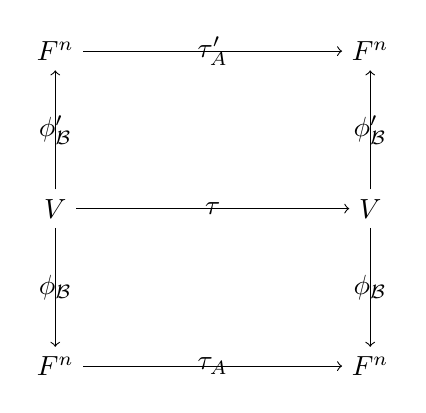
\begin{tikzpicture}
                \node(1)at(-2,0){$V$};
                \node(2)at(2,0){$V$};
                \node(3)at(-2,-2){$F^n$};
                \node(4)at(2,-2){$F^n$};
                \node(5)at(-2,2){$F^n$};
                \node(6)at(2,2){$F^n$};
                \draw[->](1)--(2)node[midway]{$\tau$};
                \draw[->](1)--(3)node[midway]{$\phi_{\mathcal{B}}$};
                \draw[->](2)--(4)node[midway]{$\phi_{\mathcal{B}}$};
                \draw[->](3)--(4)node[midway]{$\tau_A$};
                \draw[->](1)--(5)node[midway]{$\phi_{\mathcal{B}}'$};
                \draw[->](2)--(6)node[midway]{$\phi_{\mathcal{B}}'$};
                \draw[->](5)--(6)node[midway]{$\tau_A'$};
            \end{tikzpicture}
        \end{center}
    \end{sol}
\end{pf}

对 $F=\mathbb{Q}$, 由于 $\mathbb{Q}[x]$ 中的不可约多项式无次数限制, 线性算子的极小多项式可分解成任意次数不可约多项式的乘积, 此时子空间没有确定的维数, 故此时没有普适的定理.

\section{特殊的正规算子}
\begin{df}[自伴随(/厄米)算子]
    满足 $\tau=\tau^*$.
\end{df}

\begin{df}[斜伴随(/反厄米)算子]
    满足 $\tau=-\tau^*$.
\end{df}

\begin{df}[酉(/幺正)算子]
    满足 $\tau^*=\tau^{-1}$.
\end{df}

\begin{thm}[厄米算子的性质 (课本第 3 版定理 10.11)]
    $\dim V<\infty$, $\tau,\sigma\in\mathcal{L}(V)$, 则
    \begin{itemize}
        \item[(1)] 若 $\tau,\sigma$ 厄米, 则 $\tau+\sigma$, $\tau^{-1}$, $p(\tau)$ ($p(x)\in\mathbb{R}[x]$) 厄米.
        \item[(2)] $F=\mathbb{C}$, 则 $\tau$ 厄米 $\Longleftrightarrow\langle\tau(v),v\rangle\in\mathbb{R}$.
        \item[(3)] $\tau$ 为复算子或实对称算子, 则 $\tau=0\Longleftrightarrow\forall v\in V$,$\langle\tau(v),v\rangle=0$.
        \item[(4)] $\tau$ 厄米, 则 $m_{\tau}(x)$ 仅有实根.
    \end{itemize}
\end{thm}
\begin{pf}
    \begin{itemize}
        \item[(1)] $(\tau+\sigma)^*=\tau^*+\sigma^*=\tau+\sigma\Longrightarrow\tau+\sigma$ 厄米.\\
        $(\tau^{-1})^*=(\tau^*)^{-1}=\tau^{-1}\Longrightarrow\tau^{-1}$ 厄米.\\
        $p^*(\tau)=\left(\sum_ir_i\tau^i\right)^*=\sum_ir_i(\tau^i)^*=\sum_ir_i(\tau^*)^i=\sum_ir_i\tau^i=p(\tau)\Longrightarrow p(\tau)$ 厄米.
        \item[(2)] ``$\Longleftrightarrow$'': $\tau$ 厄米, 即 $\tau^*=\tau\Longleftrightarrow\forall v$, $\tau(v)=\tau^*(v)\Longleftrightarrow\langle\tau(v),v\rangle=\langle v,\tau^*(v)\rangle=\langle v,\tau(v)\rangle=\overline{\langle\tau(v),v\rangle}\Longrightarrow\langle\tau(v),v\rangle\in\mathbb{R}$.
        \item[(3)] ``$\Longrightarrow$'': 显然. 复算子的 ``$\Longleftarrow$'' 见定理 \ref{thm-9.2}, 下证实对称算子的 ``$\Longleftarrow$''.\\
        实对称算子即实厄米算子. $\because F=\mathbb{R}$, $\because\langle u,v\rangle=\langle v,u\rangle$.\\
        $\forall u,v\in V$, $0=\langle\tau(u+v),u+v\rangle=\msout{\langle\tau(u),u\rangle}0+\langle\tau(u),v\rangle+\langle\tau(v),u\rangle+\msout{\langle\tau(v),v\rangle}0=\langle\tau(u),v\rangle+\langle\tau(v),u\rangle=\langle u,\tau^*(v)\rangle+\langle\tau(v),u\rangle=\langle u,\tau(v)\rangle+\langle\tau(v),u\rangle=2\langle\tau(v),u\rangle\Longrightarrow\tau(v)=0\Longrightarrow\tau=0$.

        综上, 得证.
        \item[(4)] $\because\tau$ 厄米, $\therefore\tau$ 正规.\\
        设 $\lambda$ 为 $\tau$ 的特征值, 亦即 $m_{\tau}(x)$ 的根, 则 $\bar{\lambda}$ 为 $\tau^*$ 的特征值.\\
        $\lambda v=\tau(v)=\tau^*(v)=\bar{\lambda}v\Longrightarrow\lambda=\bar{\lambda}\Longrightarrow\lambda\in\mathbb{R}$, 故 $m_{\tau}(x)$ 仅有实根.
    \end{itemize}
\end{pf}

\begin{thm}[酉算子的性质 (课本第 3 版定理 10.12)]
    $\dim V<\infty$, $\sigma,\tau\in\mathcal{L}(V)$, 则
    \begin{itemize}
        \item[(1)] $\sigma,\tau$ 酉 $\Longrightarrow$ $r\tau$ ($\abs{r}=1$), $\sigma\circ\tau$, $\tau^{-1}$ 酉.
        \item[(2)] $\tau$ 酉 $\Longleftrightarrow\tau$ 等距同构.
        \item[(3)] $\tau$ 酉 $\Longleftrightarrow\tau$ 将一组正交归一基变换为正交归一基.
        \item[(4)] $\tau$ 酉, 则 $\tau$ 的特征值模长 $=1$.
    \end{itemize}
\end{thm}
\begin{pf}
    \begin{itemize}
        \item[(1)] $(r\tau)^*(r\tau)=\bar{r}\tau^*r\tau=\bar{r}r\tau^*\tau=\abs{r}^2\tau^{-1}\tau=1\Longrightarrow r\tau$ 酉.\\
        $(\sigma\circ\tau)^*(\sigma\circ\tau)=\tau^*\sigma^*\sigma\tau=\tau^{-1}\sigma^{-1}\sigma\tau=1\Longrightarrow\sigma\circ\tau$ 酉.\\
        $(\tau^{-1})^*=(\tau^*)^{-1}=(\tau^{-1})^{-1}\Longrightarrow\tau^{-1}$ 酉.
        \item[(2)] ``$\Longrightarrow$'': $\because$ 酉算子有逆, $\therefore$ 必双射, 下证等距.\\
        $\langle\tau(u),\tau(v)\rangle=\langle u,\tau^*(\tau(v))\rangle=\langle u,\tau^{-1}(\tau(v))\rangle=\langle u,v\rangle\Longrightarrow\tau$ 等距, 故 $\tau$ 等距同构.

        ``$\Longleftarrow$'': $\because\tau$ 等距同构, $\therefore\langle u,\tau^*(\tau(v))\rangle=\langle\tau(u),\tau(v)\rangle=\langle u,v\rangle\Longrightarrow\tau^*(\tau(v))=v\Longrightarrow\tau^*\circ\tau=1\Longrightarrow\tau$ 酉.

        综上, 得证.
        \item[(3)] ``$\Longrightarrow$'': 取一组正交归一基 $\mathcal{O}=\{o_1,\cdots,o_n\}$, $\langle o_i,o_j\rangle=\delta_{ij}$.\\
        $\because\langle\tau(o_i),\tau(o_j)\rangle=\delta_{ij}$ 且 $\dim\tau(\mathcal{O})=\dim\mathcal{O}$, $\therefore\tau(\mathcal{O})$ 为一组正交归一基.

        ``$\Longleftarrow$'': $\forall u,v\in V$, $u=\sum_{i=1}^n\alpha_io_i$, $v=\sum_{j=1}^n\beta_jo_j$.\\
        $\because\tau(\mathcal{O})$ 为正交归一基, $\therefore\langle\tau(u),\tau(v)\rangle=\langle\tau\left(\sum_{i=1}^n\alpha_io_i\right),\tau\left(\sum_{j=1}^n\beta_io_i\right)\rangle=\sum_{i,j=1}^n\alpha_i\overline{\beta_j}\langle\tau(o_i),\tau(o_j)\rangle=\sum_{i,j=1}^n\alpha_i\overline{\beta_j}\delta_{ij}=\sum_{i=1}^n\alpha_i\overline{\beta_i}=\sum_{i,j=1}^n\alpha_i\overline{\beta_j}\langle o_i,o_j\rangle=\langle\sum_{i=1}^n\alpha_io_i,\sum_{j=1}^n\beta_jo_j\rangle=\langle u,v\rangle\Longrightarrow\tau$ 等距同构 $\Longrightarrow\tau$ 酉.

        综上, 得证.
        \item[(4)] 设 $\lambda$ 为 $\tau$ 的特征值, $\tau(v)=\lambda v$, $\tau^*(v)=\bar{\lambda}v$.\\
        $v=\tau^{-1}(\tau(v))=\tau^*(\tau(v))=\bar{\lambda}\lambda v=\abs{\lambda}^2v\Longrightarrow\abs{\lambda}=1$.
    \end{itemize}
\end{pf}

\begin{thm}[正规算子的结构 (课本第 3 版定理 10.18)]
    \begin{itemize}
        \item[(1)] $F=\mathbb{C}$,
        \begin{itemize}
            \item[(a)] $\tau$ 正规 $\Longleftrightarrow\tau$ 正交归一对角化 $\Longleftrightarrow\tau$ 有正交谱分解 $\tau=\lambda_1\rho_1+\cdots+\lambda_k\rho_k$, 其中 $\lambda_i$ 互不相等, $\rho_1+\cdots+\rho_k=1$ 为单位分解, 对 $i\neq j$, $\im\rho_i\perp\im\rho_j$, $\im\rho_i\perp\ker\rho_i$.
            \item[(b)] 特征值为实数的正规算子厄米.
            \item[(c)] 特征值的模长 $=1$ 的正规算子酉.
        \end{itemize}
        \item[(2)] $F=\mathbb{R}$,
        \begin{itemize}
            \item[(a)] $\tau$ 正规 $\Longleftrightarrow V=\mathcal{E}_{\lambda_1}\odot\cdots\odot\mathcal{E}_{\lambda_k}\odot D_1\odot\cdots\odot D_l$, 其中 $D_i$ 为二维不可约的 $\tau$ 不变子空间, $D_i$ 上 $\tau$ 的矩阵表示为 $\begin{pmatrix}
                s_i&t_i\\
                -t_i&s_i
            \end{pmatrix}$.
            \item[(b)] 若上述正交直和式中无 $D_i$, 则 $\tau$ 厄米.
            \item[(c)] 若在 $D_i$ 上的 $\tau$ 的矩阵表示为 $\begin{pmatrix}
                \cos\theta&-\sin\theta\\
                \sin\theta&\cos\theta
            \end{pmatrix}$, 则 $\tau$ 酉, 称为 \textbf{正交算子}.
        \end{itemize}
    \end{itemize}
\end{thm}

\begin{df}[正交算子]
    $F=\mathbb{R}$ 的酉算子.
\end{df}

\section{(半)正定算子}
\begin{df}[(半)正定算子]
    $F=\mathbb{R}$, $\dim V<\infty$, $\tau\in\mathcal{L}(V)$ 厄米, 若 $\forall v\in V$, $\langle\tau(v),v\rangle>(\geq)0$, 则 $\tau$ \textbf{(半)正定}.
\end{df}

\begin{thm}[(课本第 3 版定理 10.22)]
    $F=\mathbb{R}$, $\dim V<\infty$, $\tau\in\mathcal{L}(V)$ 厄米, 则
    \begin{itemize}
        \item[(1)] $\tau$ 半正定 $\Longleftrightarrow\tau$ 的特征值 $\geq 0$.
        \item[(2)] $\tau$ 正定 $\Longleftrightarrow\tau$ 的特征值 $>0$.
    \end{itemize}
\end{thm}
\begin{pf}
        ``$\Longrightarrow$'': 设 $\lambda$ 为 $\tau$ 的特征值.\\
        $\because\tau$ (半)正定, $\therefore\langle\tau(v),v\rangle>(\geq)0$.\\
        又 $\because\langle\tau(v),v\rangle=\langle\lambda v,v\rangle=\lambda\langle v,v\rangle\geq 0$, $\langle v,v\rangle>0$, $\therefore\lambda>(\geq)0$, $\therefore\lambda>(\geq)0$.

        ``$\Longleftarrow$'': $\because\rho$ 厄米, $\therefore\tau$ 的正交谱分解 $\tau=\lambda_1\rho_1+\cdots+\lambda_k\rho_k$.\\
        对 $\tau$ 的函数操作均等效于作用于其谱分解的特征值上: $\tau^2=\sum_{ij}\lambda_i\lambda_j\rho_i\rho_j=\sum_{ij}\lambda_i\lambda_j\delta_{ij}\rho_i=\sum_i\lambda_i^2\rho_i$.\\
        类似地, $\tau^k=\sum_{i}\lambda^k\rho_k$.\\
        $r\tau^k=r\sum_i\lambda_i^k\rho_i=\sum_ir\lambda_r^k\rho_i\Longrightarrow$ 对 $f(x)\in F[x]$, $f(\tau)=\sum_if(\lambda_i)\rho_i$,\\
        $\forall$ 可由多项式近似的 $g(x)$, $g(\tau)=\sum_ig(\lambda_i)\rho_i$.\\
        $\because\tau$ (半)正定, $\therefore$ 必可定义其平方根 $\sqrt{\tau}=\sqrt{\lambda_1}\rho_1+\cdots+\sqrt{\lambda_k}\rho_k$, 此处 $\lambda_i>(\geq)0$, 否则 $\sqrt{\tau}$ 不一定合法.
\end{pf}

\begin{thm}[(课本第 3 版定理 10.23)]
    $\tau$ 厄米, 则
    \begin{itemize}
        \item[(1)] $\tau$ 半正定 $\Longleftrightarrow\tau$ 有平方根.
        \item[(2)] $\tau$ 半正定 $\Longleftrightarrow$ $\tau=\sigma^*\circ\sigma$, 其中 $\sigma\in\mathcal{L}(V)$ (注意这里的 $\sigma$ 不唯一).
    \end{itemize}
\end{thm}
\begin{pf}
    \begin{itemize}
        \item[(1)] $\tau$ 半正定, 即 $\tau=\sum_i\lambda_i\rho_i$, 其中 $\lambda_i\geq 0\Longleftrightarrow\sqrt{\tau}=\sum_ir_i\rho_i$, 其中 $r_i=\sqrt{\lambda_i}$.
        \item[(2)] ``$\Longrightarrow$'': 取 $\sigma=\sqrt{\tau}$ 即得证.

        ``$\Longleftarrow$'': $\langle\tau(v),v\rangle=\langle\sigma^*\circ\sigma(v),v\rangle=\langle\sigma(v),\sigma(v)\rangle=\norm{\sigma(v)}^2\geq 0\Longrightarrow\tau$ 半正定.
    \end{itemize}
\end{pf}

\begin{thm}[半正定算子的复合半正定的条件 (课本第 3 版定理 10.24)]
    $\sigma,\tau\in\mathcal{L}(V)$ 半正定, 若 $\sigma\circ\tau=\tau\circ\sigma$, 则 $\sigma\circ\tau$ 半正定.
\end{thm}
\begin{pf}
    $\because\sigma\tau=\tau\sigma$, $\therefore\sqrt{\sigma}\sqrt{\tau}=\sqrt{\tau}\sqrt{\sigma}\Longrightarrow\sigma\tau=\sqrt{\sigma}\sqrt{\sigma}\sqrt{\tau}\sqrt{\tau}=(\sqrt{\sigma}\sqrt{\tau})(\sqrt{\sigma}\sqrt{\tau})$, 故 $\sigma\tau$ 半正定.
\end{pf}

\section{算子的极分解}
\begin{thm}[算子的极分解 (课本第 3 版定理 10.25)]
    $F=\mathbb{C}$, 有限维内积向量空间 $V$, $\tau\in\mathcal{L}(V)$, 则 $\exists!$ 半正定算子 $\rho$ 及酉算子 $\nu$, s.t. $\tau=\nu\circ\rho$, 且若 $\tau$ 可逆, 则 $\nu$ 唯一.
\end{thm}
\begin{pf}
    \begin{itemize}
        取 $\rho=\sqrt{\tau^*\tau}$, 则 $\norm{\rho(v)}^2=\langle\rho(v),\rho(v)\rangle=\langle v,\rho^*\rho(v)\rangle=\langle v,\rho^2(v)\rangle=\langle v,\tau^*\tau(v)\rangle=\langle\tau(v),\tau(v)\rangle=\norm{\tau(v)}^2$.\\
        取 $\nu:\im\rho\rightarrow\im\tau$, $\rho(v)\mapsto\tau(v)$.\\
        先证 $\nu$ 为映射: 若 $\rho(v)=\rho(u)$, 则 $\rho(u-v)=0\Longrightarrow\norm{\rho(u-v)}^2=0\Longrightarrow\norm{\tau(u-v)}=^2=\langle\tau(u-v),\tau(u-v)\rangle=0\Longrightarrow\tau(u-v)=0\Longrightarrow\tau(v)=\tau(u)$, 故 $\nu$ 为映射.\\
        $\because\norm{\nu(\rho(v))}=\norm{\tau(v)}=\norm{\rho(v)}$, $\therefore\nu$ 等距同构 $\Longrightarrow\nu$ 酉.

        当 $\tau$ 不可逆时, 拓展 $\im\rho$ 为 $\im\tau$ 的方式不唯一, 故 $\nu$ 不唯一.
    \end{itemize}
\end{pf}

若 $\sigma$ 酉, 则其特征值模 $\abs{\lambda}=1$, 可记为 $\lambda_i=e^{i\theta_i}$, 其中 $\theta_i\in\mathbb{R}$,\\
则 $\sigma=\lambda_1\rho_1+\cdots+\lambda_k\rho_k=e^{i\theta_1}\rho_1+\cdots+e^{i\theta_k}\rho_k$, 其中 $\rho_1+\cdots+\rho_k=1$ 为正交单位分解.\\
令 $H=\theta_1\rho_1+\cdots+\theta_k\rho_k$, 则
\begin{itemize}
    \item[(1)] $H^*=H$.
    \item[(2)] $\sigma=e^{iH}$.
\end{itemize}
此处 $H$ 类似量子力学中的哈密顿量, $\sigma$ 类似演化算子.
\ifx\allfiles\undefined
\end{document}
\fi
